\subsection{问题三分析}
\subsubsection{排队模型}
\begin{defnbox}{排队模型}{queue}
    排队系统主要由输入过程、排队规则和服务机构构成。输入过程,即顾客到来的时间规律,出租车辆到达的时间规律常被视为服从泊松分布;排队规则,即顾客以何种规则排队,可分为损失制、等待制、混合制;服务机构,可分为单服务台、多服务台并/串联、混合型;服务规则多样,有先到先得、后到先得、随机服务、优先服务等规则。其表示方式为:\verbbox{X/Y/Z/A/B/C}。其中,
    \begin{itemize}
        \item \verbbox{X}表示顾客到达流或顾客到达间隔时间的分布;
        \item \verbbox{Y}表示服务时间的分布;
        \item \verbbox{Z}表示服务台数目;
        \item \verbbox{A}表示系统容量限制;
        \item \verbbox{B}表示顾客源数目;
        \item \verbbox{C}表示服务规则。
    \end{itemize}
\end{defnbox}

定义$\lambda$为单位时间车辆平均到达率,$\mu$为单位时间系统服务率, 定义$\rho$为服务强度,$\rho=\lambda/\mu$。$\rho<1$, 则系统服务率大于车辆平均到达率满足服务要求,反之不能满足。

\verbbox{M/M/1}(单点式排队系统)排队模型认为车辆的到达服从泊松分布,出租车服务时间服从负指数分布,仅有一个服务台服务。布局形式如图~\ref{fig:MM1_draw}。\verbbox{M/M/S}模型则有多个服务台服务。

\begin{itemize}
    \item 单点式出租车排队服务系统是指一列乘客等候上车的队伍对应一个上车点的布局形式;
    \item 多点纵列式出租车排队服务系统属于面向乘客的带有多个服务台和一个公共队伍的排队系统;
    \item 多点并列式出租车排队服务系统与多点纵列式类似,但系统内各个上车点的布置形式呈并列式。
\end{itemize}

\subsubsection{三种常见的服务布局对比}

详见表格~\ref{tab:taxi-queue-dis-advantage}

\begin{table}
    \centering
    \resizebox{\textwidth}{!}{%
        \begin{tabular}{cccc}
            \toprule
             & 优点 & 缺点 & 适用环境 \\ \midrule
            \rowcolor[HTML]{EFEFEF}
            单点式(如图~\ref{fig:MM1_draw}) & \begin{tabular}[c]{@{}c@{}}造价低;\\ 安全,乘客与出租车\\ 同时在各自的等候空\\ 间进行排队。\end{tabular} & \begin{tabular}[c]{@{}c@{}}等候时间长,只有当\\ 一个乘客服务结束离\\ 开排队系统后,后面\\ 的乘客才能接受服务。\end{tabular} & \begin{tabular}[c]{@{}c@{}}客源较少的小型\\ 枢纽站的出租车\\ 上客区或者路侧\\ 出租车服务点。\end{tabular} \\
            多点纵列式(如图~\ref{fig:juxtaMM1}) & \begin{tabular}[c]{@{}c@{}}增加了上车服务点,\\ 提高了系统的服务效\\ 率。\end{tabular} & \begin{tabular}[c]{@{}c@{}}多个服务点的出租车\\ 同时驶离各自的上车\\ 点时,车辆之间易产\\ 生干扰与冲突。\end{tabular} & \begin{tabular}[c]{@{}c@{}}机场等枢纽的纵\\ 向距离较大的交\\ 通枢纽。\end{tabular} \\
            \rowcolor[HTML]{EFEFEF}
            多点并列式(如图~\ref{fig:juxtaMM2}) & \begin{tabular}[c]{@{}c@{}}分散客流,乘客离站\\ 效率提高。\end{tabular} & \begin{tabular}[c]{@{}c@{}}容易产生客流干扰及\\ 人车冲突。\end{tabular} & \begin{tabular}[c]{@{}c@{}}上客区纵向距离\\ 较短的传统枢纽。\end{tabular} \\ \bottomrule
        \end{tabular}%
    }\caption{不同出租车排队服务系统的优缺点}\label{tab:taxi-queue-dis-advantage}
\end{table}

\begin{figure}
    \centering
    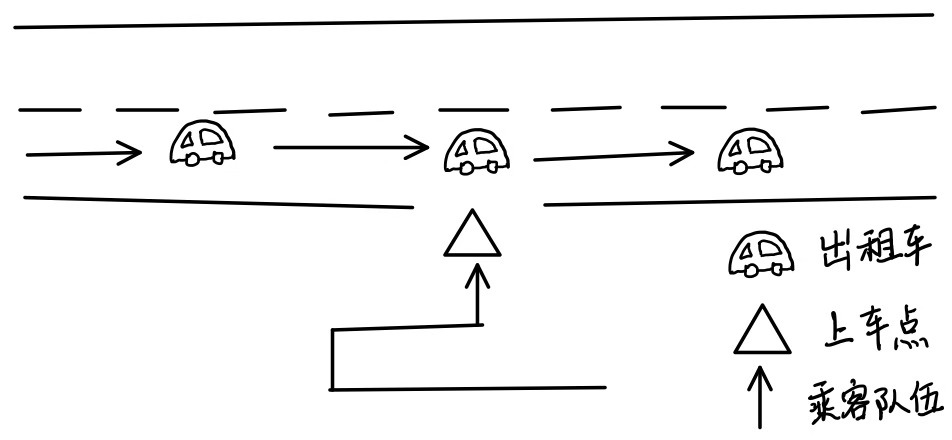
\includegraphics[width=.6\textwidth]{MM1_draw.jpg}
    \caption{\texttt{M/M/1}出租车排队服务布局}\label{fig:MM1_draw}
\end{figure}

\begin{figure}
    \centering
    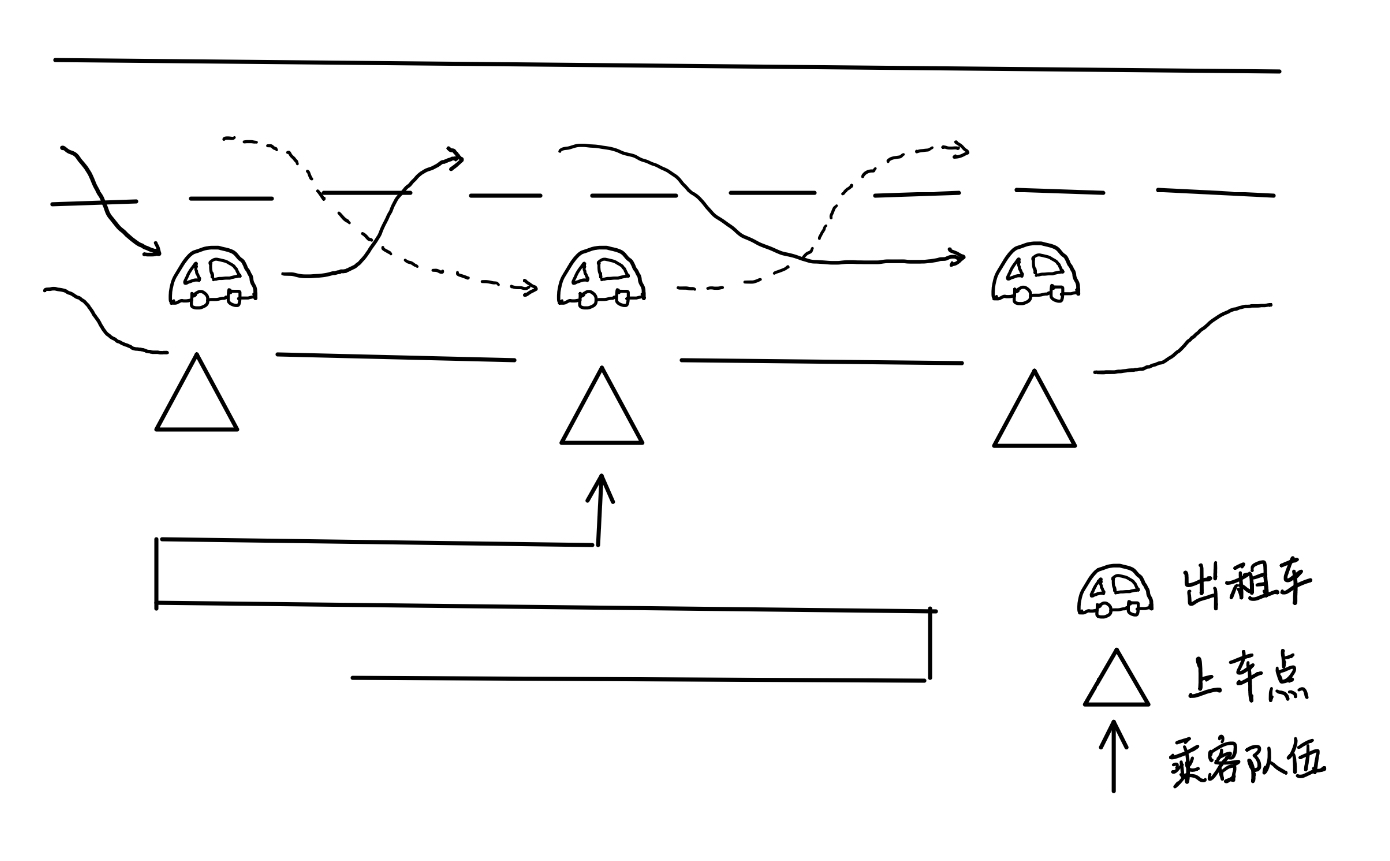
\includegraphics[width=.6\textwidth]{juxtaposeMM1.jpg}
    \caption{纵列\texttt{M/M/S}出租车排队服务布局}\label{fig:juxtaMM1}
\end{figure}

\begin{figure}
    \centering
    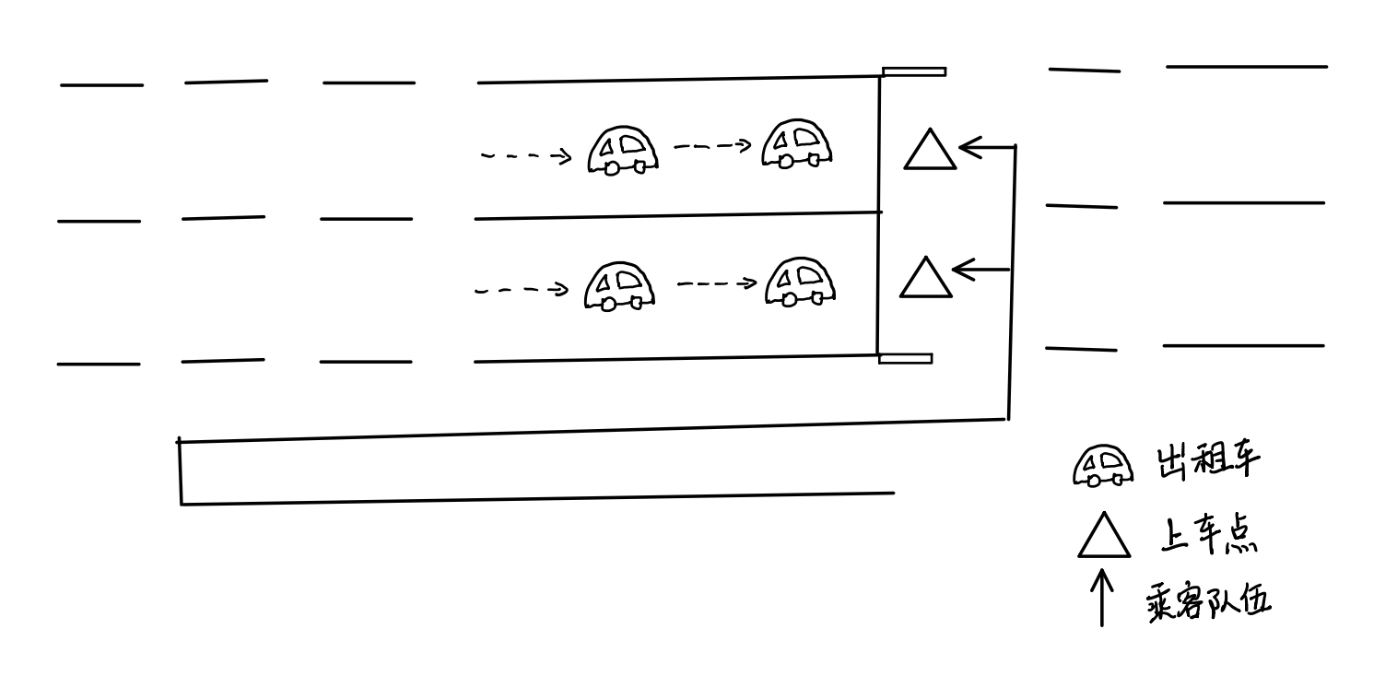
\includegraphics[width=.6\textwidth]{MM2.jpg}
    \caption{并列\texttt{M/M/S}出租车排队服务布局}\label{fig:juxtaMM2}
\end{figure}



\begin{figure}
    \centering
    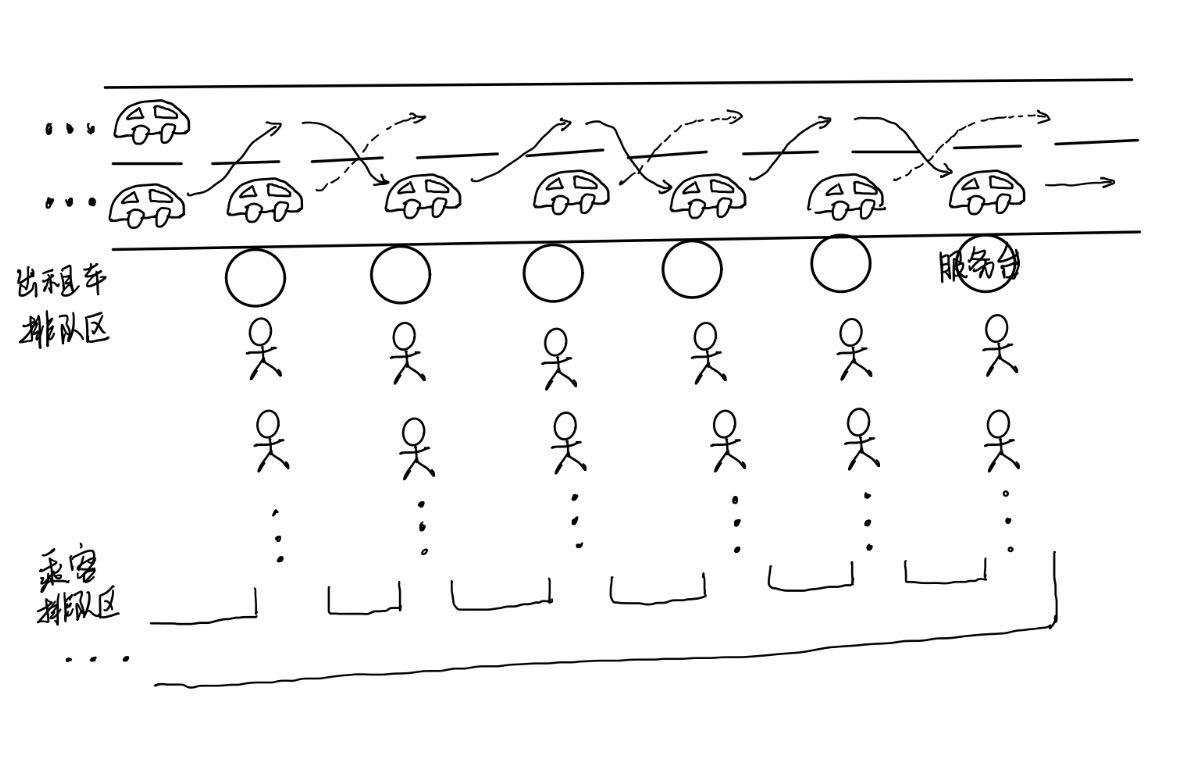
\includegraphics[width=.6\textwidth]{conclusion.jpg}
    \caption{问题三的解决方案设计简图}\label{fig:conclusion}
\end{figure}




%\begin{figure}
 %   \centering
  %  \begin{minipage}[c]{0.48\textwidth}
   %     \centering
    %    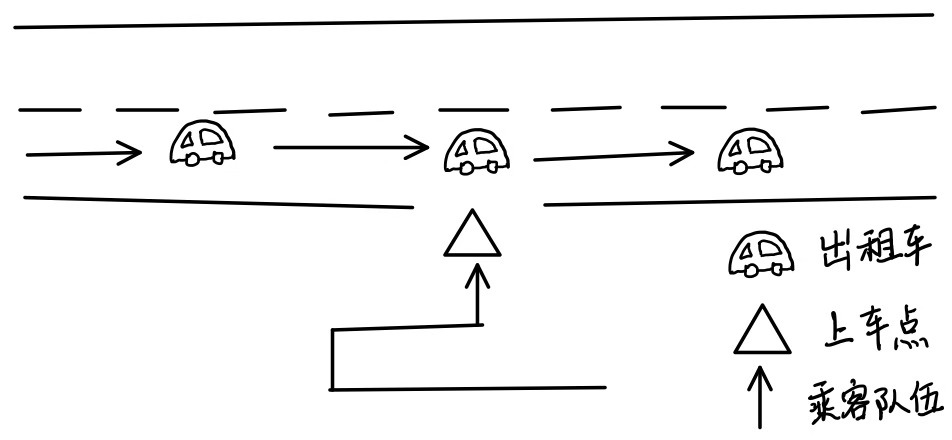
\includegraphics[height=0.2\textheight]{MM1_draw.jpg}
     %   \subcaption{M/M/1出租车排队服务布局}
    %\end{minipage}
    %\begin{minipage}[c]{0.48\textwidth}
    %    \centering
    %    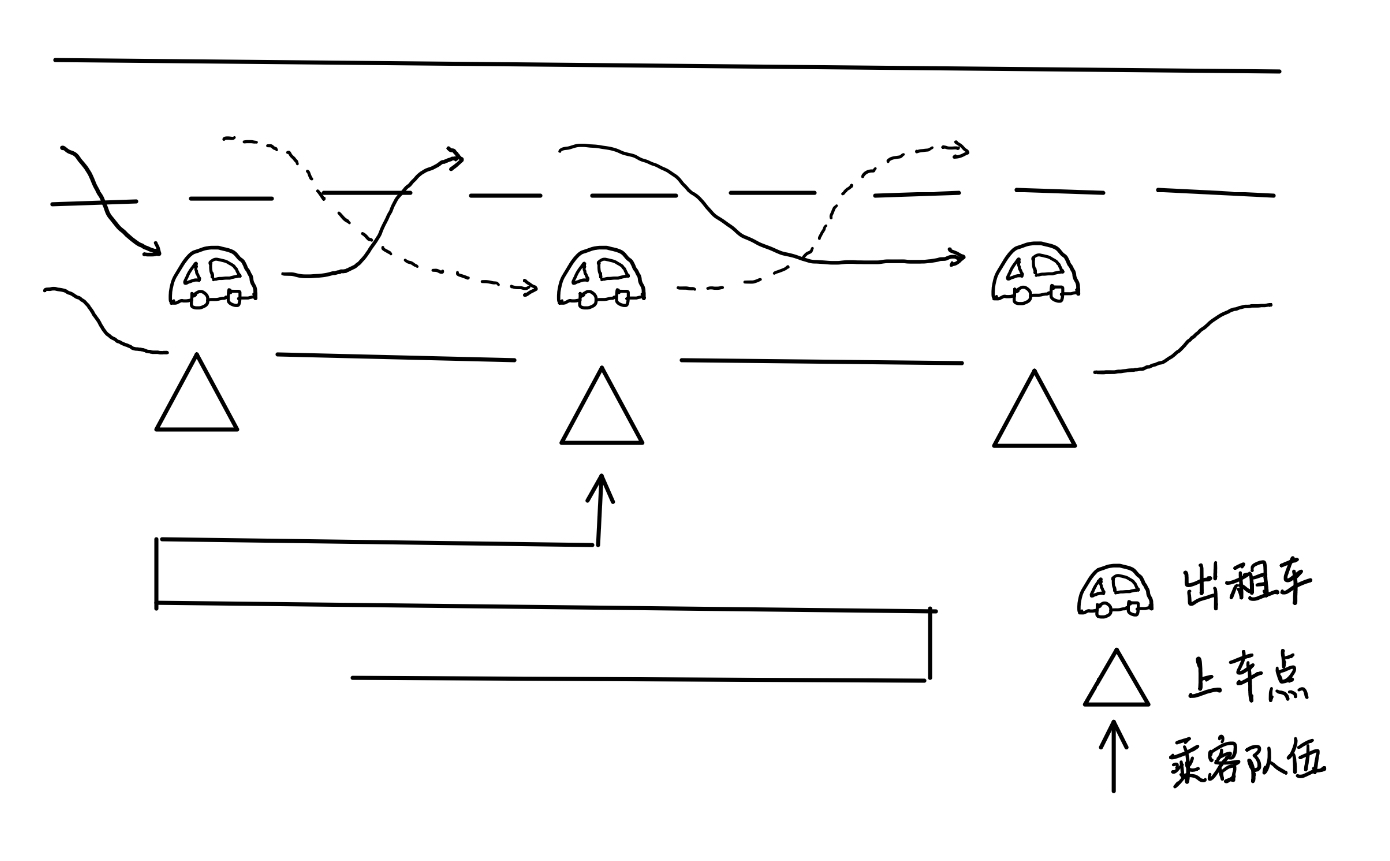
\includegraphics[height=0.2\textheight]{juxtaposeMM1.jpg}
    %    \subcaption{并列M/M/S出租车排队服务布局}
    %\end{minipage}
    %\caption{出租车排队服务系统}
%\end{figure}

\subsection{排队模型建立}
根据排队论的相关理论,对枢纽内多点式出租车上客区这一排队系统建立排队模型 。当上客区排队系 统处于全忙期,且系统的服务强度$ρ< 1$时,系统达到稳定状态且不会形成无限排队的现象,在此基础上对系统的输入与输出进行建模。

在系统达到稳态时,$C$个服务台工作,系统中出租车乘客数为$n$的概率如下:
\begin{equation}\label{eq:排队系统出租车乘客数0}
    P_0(C) = \left[\sum_{k=0}^{C-1}\frac{1}{k!}\left(\frac{\lambda}{\mu}\right)^k+ \frac{1}{C!}\frac{1}{(1-\rho)}\left(\frac{\lambda}{\mu}\right)^C\right]^{-1}
\end{equation}

\begin{equation}\label{eq:排队系统出租车乘客数n}
    P_n(C) = \begin{cases}
        \left(\lambda/\mu\right)^kP_0(C)/n, & n=1, 2, \ldots, C \\
        \left(C!C^{n-C}\right)^{-1}\left(\lambda/\mu\right)P_0(C), & n=C+1
    \end{cases}
\end{equation}

用系统中乘客排队的队长$L_s$及其逗留时间$W_s$对系统进行分析,得:
\begin{equation}\label{eq:排队系统乘客队长-2}
    L_s = L_q + C_\rho = \frac{1}{C!}\frac{(C\rho)^C\rho}{(1-\rho)^2}P_0 + \frac{\lambda}{\mu},
\end{equation}

\begin{equation}\label{eq:排队系统逗留时间}
    E(W_s) = \frac{P_n(C)}{C\mu(1-\rho)^2} = \frac{n\mu}{n!(n\mu-\lambda)^2}\left(\frac{\lambda}{\mu}\right)^nP_0(C).
\end{equation}


\subsection{排队系统优化}
利用排队系统的费用决策模型对排队系统进行优化设计。假设乘客等待时间的总费用为$Z_1=\alpha L_s$ ,上车点建设成本为$Z_2=\beta C$,其中$\alpha$为每个乘客单位时间的等待时间成本,$\beta$为单个服务台的服务时间成本与单个上车点的建设费用。当则需要满足两者之和最小才能使得系统进一步优化,即:
\begin{equation}\label{eq:最小化成本}
    \min:Z(C) = Z_1 + Z_2 = \alpha L_s(C) + \beta C, \quad Z(C-1)\leq Z(C)\leq Z(C+1)
\end{equation}

\subsection{结论}
在解决本问题时,对国内各交通枢纽已有的服务布局进行了调研,并总结出了最常见的三种进行分析讨论。并以深圳机场及题目要求为例,对多点式的排队服务系统进行了评析。利用排队论中的费用决策模型对排队系统进行优化,设计方案如图~\ref{fig:conclusion}。经过调查与计算得,当上客区的上车点数为6,即设置6个可同时搭载乘客的出租车候客服务台时,乘客排队等待时间成本与车道设置成本之和构成的总费用最小。
